\documentclass[11pt,a5paper]{book}
\usepackage[utf8]{inputenc}
\usepackage{amsmath}
\usepackage{amsfonts}
\usepackage{amssymb}
\usepackage{graphicx}
\usepackage[super]{nth}
\usepackage{float}

\title{Navigating Fisheries Assessments}
\author{Marcel Gietzmann-Sanders}
\date{}
\setcounter{tocdepth}{1}
\begin{document}
\maketitle
\newpage

One day I downloaded an Atlantic Herring Stock Assessment. Then I looked at the page count. Over 300 pages of delicious technical detail. That's when I realized I needed a map. This is the first one. Hope it helps.

\tableofcontents
\newpage

\chapter{Well What's the Point?}

Quantitative fisheries science (hereafter referred to just as fisheries modeling) is all about the following question:
\newline

\hangafter=0 \hangindent=1cm \noindent How can a fishery bring the most long term benefit to society?
\newline

Nice and clear, right? Hardly. This is one of those wonderfully simplistic statements that throws a veil of apparent clarity over an entangled mass of delicious complexity. In other words, there's a lot to unpack.
\newline

Like all such statements it takes only the most rudimentary of questions to blow its cover. For example - what is a fishery? That's a question biologists are still arguing about and in all likelihood we've been fishing since before the invention of fire itself! 
\newline

Fortunately humans are pretty good at pretending the world is a lot simpler than it is and somehow managing to get away with it. Abstraction is a rather powerful tool of ours.
\newline

That being said the fun in a question like this one is not the abstraction itself but in the mind opening richness that comes from unraveling it.
\newline

So let's do some unraveling shall we? 
\newpage

\noindent \rule{\textwidth}{0.5pt} 
\noindent How can a \textbf{fishery} bring the most long term benefit to society?
\newline
\rule{\textwidth}{0.5pt} 
\vspace{5pt}

I know what you're thinking. Didn't I just say that no one's actually been able to agree on what a fishery \textit{exactly} is? How on earth then do I suppose I'm about to answer the question myself? 
\newline

Well see, if I don't at least present a working definition... well... then we'll have nothing to work with and this whole exploration of fisheries science will be rather short. So consider this definition less of an audacious claim of certainty on my part and more of a desperate attempt to find some common ground for us to stand on. 
\newline

Alright, here goes. A fishery in this book is going to mean a specific group of marine populations, at least one of which we catch and use. This definition is nice because it allows for both ecosystem based management (multiple interacting populations) and more tradition forms of management that work with one species at a time. 
\newline

That being said it's worth noting that I'm looking at the population as a whole. And that means I'm roping in \textit{everyone} who touches it. Unintended catch (bycatch), intended catch, commercial, recreational, artisinal, I'm throwing them all in the same... well... boat. I think as we pull the thread and unravel this problem it will become clear why I've decided to do this, but just be warned that to others a fishery can mean quite the opposite. Instead of focusing on the population such definitions often focus on the humans fishing it. 
\newpage

\noindent \rule{\textwidth}{0.5pt} 
\noindent How can a fishery bring the most long term \textbf{benefit} to society?
\newline
\rule{\textwidth}{0.5pt} 
\vspace{5pt}

If defining a fishery was difficult, defining what benefit to society means is even more so. Which is why I'm just not going to bother.
\newline

At least not now.
\newline

Benefits to society are marvelously specific to the fishery in question. These boons can be nutritional, cultural, financial, ecological, spiritual... yea you get the idea. Fisheries can make or break communities, they provide medical inputs, represent a multi-billion dollar industry, provide a primary source of protein to a good half of the entire world population, and are, quite critically, an essential part of an unnerving proportion of my lunches (although I may be a bit biased on that last point).
\newline

My point is simple - benefits cannot be defined in the abstract, you have to get down and dirty to \textit{really} understand what a fishery does and what it can mean to society. 
\newline

\textit{Know thy fishery}.
\newpage


\noindent \rule{\textwidth}{0.5pt} 
\noindent How can a fishery bring the most \textbf{long term} benefit to society?
\newline
\rule{\textwidth}{0.5pt} 
\vspace{5pt}

The need for food is one of those things that just doesn't go away. No matter how many times you eat, no matter how excellent the food, you always end up hungry a few hours later. It's just life. As such fisheries have to be sustainable - they \textit{need} to be able to bring in food year after year after year. And this often leads to a pill that's hard to swallow - in order to not burn out one has to slow down. (And that's a bit of wisdom that applies to a lot more than just catching fish). \newline

Each and every fishery must sort out not just how to bring benefit but how to guarantee that benefit to all those who will inherent the earth.
\newpage


\noindent \rule{\textwidth}{0.5pt} 
\noindent How can a fishery bring the \textbf{most} long term benefit to society?
\newline
\rule{\textwidth}{0.5pt} 
\vspace{5pt}

This now, well this is the question that brings out the pitchforks, firebrands, and lobbyists. It's one thing to acknowledge all the benefits a fishery can bring to society - figuring out how to balance all of these value propositions is quite another thing. Beyond struggling with the question of who society is and how to make sure it is represented, this balancing act may be the single most important activity in fisheries management which is exactly why I'm not going to attempt to answer the question at all. 
\newline

I am not judge, jury, and executioner - I'm just a dude who likes fish, numbers, and environmental stewardship. But suffice it to say, fisheries scientists have a \textit{responsibility} to help ensure that the political conversation is as data driven as possible and help create win-win situations whenever possible. These kinds of things tend to pit folks against each other and arch-nemeses make for incredible blinders.
\newline

Just as importantly it's paramount that every fisheries scientist out there recognizes that while their science may seem impartial or whatever there is always an implicit balance of benefits in every single optimization we ever do. That's a hard truth one can never escape. Know what you're fighting for because any and all data represents ammunition for someone. 
\newpage

\noindent \rule{\textwidth}{0.5pt} 
\noindent \textbf{How} can a fishery bring the most long term benefit to society?
\newline
\rule{\textwidth}{0.5pt} 
\vspace{5pt}

Obviously there are loads of ways to improve the benefits to society. Finding better ways to fish, setting catch limits to prevent the merciless decimation of a fish stock, being smarter about what's taken and what's left to breed and grow - these are some of the more apparent ones. However there are loads of other ways to hack the value of fisheries - becoming a restaurateur who changes public opinion about a specific species of fish, developing monitoring for the supply chain to help people understand where their food is coming from, or finding new ways to farm fish - there are a lot of really cool and interesting options. 
\newline

However I know I've got limited time with you and so, for the sake of brevity, I'm going to have to limit scope. So we're going to focus on being creative about the actions the fishers themselves can take when they're out actually catching the fish. For the full range of ingenious action that can be taken I refer you to the rich literature surrounding fisheries. 
\newpage

\noindent \rule{\textwidth}{0.5pt} 
\noindent  How can a fishery bring the maximum long term benefits to \textbf{society}?
\newline
\rule{\textwidth}{0.5pt} 
\vspace{5pt}

This is a question with an obvious answer that probably should be paid more attention to. Society is \textit{all} of us. It's not just mega-corps, it's not just the town near the fish that's been fishing there for centuries, and its not limited to the consumer either. It is \textit{everyone} and making sure \textit{all} are represented is of utmost importance. 
\newline

And as with the "most" question each and every model we build, each optimization we run, has implicit notions about \textit{who} society is. Be conscientious of that. 
\newpage

Alright, with all of that in mind I think our question is looking a little bit different. 
\newline

\hangafter=0 \hangindent=1cm \noindent \textbf{Fisheries modeling is about informing the set of fishing practices that would maximize a specific balance of benefits in a sustainable fashion. This information should then be used as part of a representative collaboration to find the balance best suited to the whole.}
\newline

So, what's needed to make this happen? Well wouldn't you know? By a wonderful coincidence that just happens to be what the next section is about. 
\newpage

\chapter{The 30,000 Foot View}

\noindent \rule{\textwidth}{0.5pt} 
\begin{figure}[h!] 
  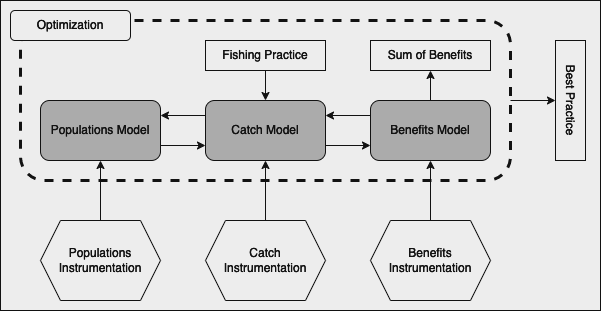
\includegraphics[width=\linewidth]{drawings/high_level_models.png}
  \caption{Models}
  \label{fig:high_level_models}
\end{figure}
\newline
\rule{\textwidth}{0.5pt} 
\vspace{5pt}

To optimize requires predicting things that have never happened (and likely never will). Doing so requires mathematical models that give you the confidence to wade into the unknown. And for our particular problem those models split into three broad categories - benefits, population, and catch. 
\newline

The benefits model is exactly what it sounds like - it's how we derive the long term benefit. For example, if the \textit{only} benefit under consideration is a price that happens to be based on the weight of the fish caught (where more is not always better) then part of our benefit model would be a curve that ties a fish's weight to expected price. The other building block of our model would be a procedure for applying this curve across the catch from each consecutive year. Integrate this across the years with some temporal amortization and you've got a long term benefits forecast. 
\newline

All this is great, but means rather little if you've got no sense of the underlying fish population. Right away then we bump into the population model. A population has but one (very complicated) job - to tell us how the population will develop over time given the environment it finds itself in. These models can include such things as where the fish like to get it on, how their young end up getting back into the general population, how quickly and to what perils the fish die as the years go on, as well as things like how years spent being a fish turn into length and weight, whether fish from one population interact their brethren from other populations, and who to watch out for if you're a fish closer to the bottom of the food chain. Population models get wildly interesting and include loads of biological and ecological knowledge. 
\newline

Alright, so in one hand we have a model relating the fish caught to the rewards reaped and in the other hand we've got a model of the population dynamics driving the ever shifting ecology of the fish world. In between them stands the main act - the reason we're all here - the catch itself. And just like the catch connects the fish population to our dinner plates, so too does the catch model connect our population models to the benefits models. However, this model holds a very special place, because it is this model that has the dials we turn to try and optimize fishing practice. Think of the other models as like the engine, transmission and wheels of a vehicle, present, important, but ultimately deterministic machinations beyond our direct control. Instead it is through the medium of gear lever, pedals, and steering wheel that we guide the mechanism forward. In like manner the catch model is how we drive the fisheries mobile to (hopefully) better days. 
\newpage

\noindent \rule{\textwidth}{0.5pt} 
\begin{figure}[h!] 
  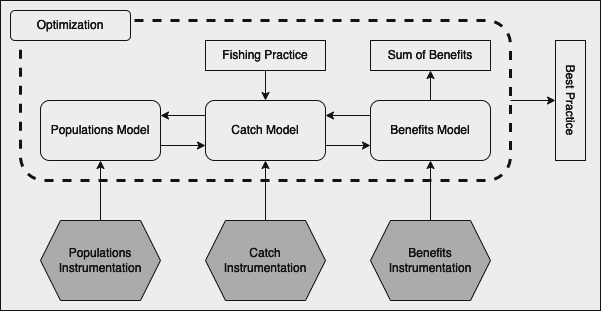
\includegraphics[width=\linewidth]{drawings/high_level_instrumentation.png}
  \caption{Instrumentation}
  \label{fig:high_level_instrumentation}
\end{figure}
\newline
\rule{\textwidth}{0.5pt} 
\vspace{5pt}

We've been talking about models quite flippantly. That's the nice thing about abstractions, you can talk about them as if they are but an arm's reach away, just ready to be plucked out of the mental sky of the imagination. Reality is rarely so kind. Models are monsters. Glorious to behold, tricky to master, and devilishly hard to train, they require significant expertise and thought to get right. But in and amongst all of their diversity there is one thing all models share - models must be fit.
\newline

Now by that I don't mean models need to be burly or able to run a race in a specific period of time, what I mean is that models have to fit in - you must look at them and see nothing but reality itself. And fitting a model is one of those things that while easy enough to explain is devilishly hard to do. 
\newline

So in the usual fashion, let's do the easy part - the explaining. 
\newline

Let's use a simple example. Fisheries scientists often have to model the relationship between age $t$ and length $L$. One one such model is the Von Bertalanffy growth curve:

$$L = L_{\infty}(1-e^{-Kt})$$

This equation is pretty straight forward. That exponential term, the $e^{-Kt}$, will, assuming $K>0$, go to zero as $t$ gets larger and larger. And that means that as the years go by $L$ becomes more and more like $L_{\infty}$. To put this more plainly growth starts out quickly and then slows down over time until it becomes barely perceivable, maxing out at this imaginary $L_{\infty}$ - the length of an infinitely old fish (who knows, perhaps some deity keeps pets). 
\newline

Whether or not you believe fish grow this way is irrelevant, it's just an illustration of fitting after all. And like all good simple examples it paints a nice clear point. The point is that this model, like all other models out there, has three main components - input variables - $t$, output variables - $L$, and parameters - $L_{\infty}$ and $K$. 
\newline

The way you use the model is also straightforward - you get some measurements, plug them into your input variables, run the equation, and get some predictions as the output variables. Easy peasy. 
\newline

There is a problem however - none of this is going to work if we don't know what $K$ and $L_{\infty}$ should be. This is where the fitting comes in. To build any model you have to have some situations in which both the input and output variables are known. Then you can choose the parameters that best fit that "ground truth" data. 
\newline

For example (I know, examples within examples!), suppose our measured ground truth looked something like Fig. \ref{fig:length_measurements_by_year}.
\newline


\begin{figure}[h!] 
  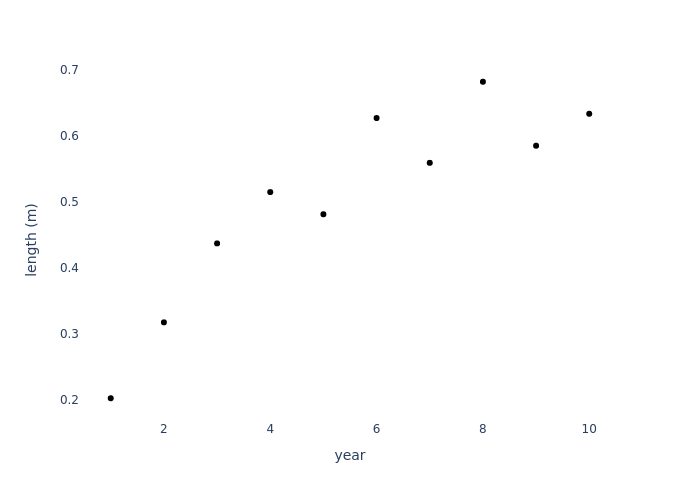
\includegraphics[scale=0.35]{notebooks/Fitting/new_measurements.png}
  \caption{Average Length Measurements by Year}
  \label{fig:length_measurements_by_year}
\end{figure}

First we can note that our measurements never exceed 0.7. So I'd say a pretty good guestimate for $L_{\infty}$ would be just that - 0.7.  Then we can try a few examples of $K$ and see what works well.
\newline

\begin{figure}[h!] 
  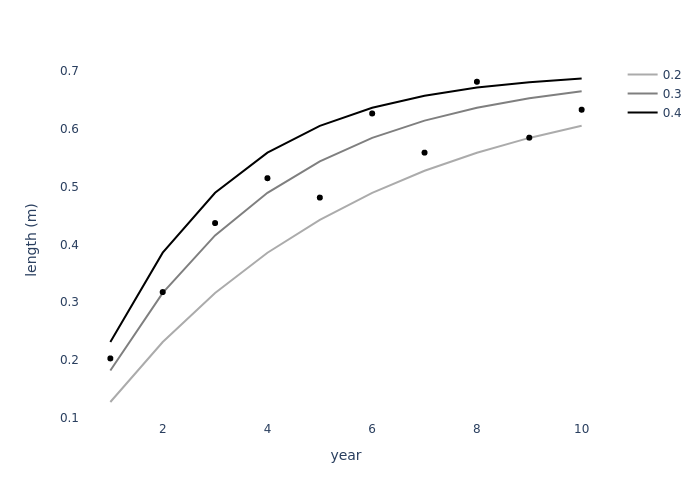
\includegraphics[width=\linewidth]{notebooks/Fitting/fit_lines.png}
  \caption{Attempting to Fit $K$}
  \label{fig:fitting_K}
\end{figure}

Fig. \ref{fig:fitting_K} shows us the predicted length vs year relationship for three values of $K$ - 0.2, 0.3, and 0.4. By just visual inspection we can see that 0.2 doesn't grow fast enough whereas 0.4 grows to quickly, so 0.3 is probably a reasonable fit.
\newline

How did I guess these? Well I built the example of course! Unfortunately we are rarely in possession of such retrospective knowledge and so mathematicians, scientists, and computer scientists have come up with loads of automated mechanisms for fitting parameters. (An absolutely fascinating subject by the way. If we had more time I would definitely nerd out about it). 
\newline

So in sum, to fit a model you need, ground truth data, a mechanism for arriving at the fit, and... well... the model is also pretty handy to have on hand. We have the model, folks have built the mechanisms for automatically tuning it, and so what's missing is the ground truth data. 
\newline

These data and the instrumentation and labor that goes into collecting it are the unsung heroes of the modeling world. Everyone loves to talk about the new artificial intelligence they just breathed life into, or how by switching models some prior, dubious assumptions could be relaxed, but none of that would be possible without the data. And that's why in my diagram they get their own special place.
\newpage

\noindent \rule{\textwidth}{0.5pt} 
\begin{figure}[h!] 
  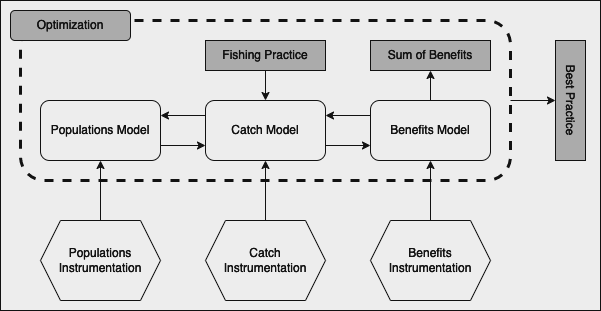
\includegraphics[width=\linewidth]{drawings/high_level_optimization.png}
  \caption{Optimization}
  \label{fig:high_level_optimization}
\end{figure}
\newline
\rule{\textwidth}{0.5pt} 
\vspace{5pt}

Voila! We've got ourselves some models that, thanks to our stunning ground truth data have been fit to look convincing like our earthly reality. Now what? Well to lean on my dodgy analogy from before, it's time to grab the steering wheel, hit the gas, and drive the fisheries mobile to a better tomorrow. To get a sense of what it's like to get behind the wheel let's once again turn to a simple(ish) example. 
\newline

All optimizations begin with taking the knobs we intend to turn and quantifying them. In our case, to keep things clear, we're going to assume that we're just directly controlling fishing mortality $F$ (and yes, I admit, I have no idea how you'd actually control such a thing directly). 
\newline

Next we know we need to start with our models and we may as well begin with the population side of things. Let the sweeping assumptions begin!
\newline

First we're going to assume that the fish population dies off in strict accordance to a mathematical equation (cold? I suppose so):

$$\frac{dN}{dt}=-ZN$$

How to read this? It just says that the \textit{instantaneous} decrease in fish is proportional to the number of fish present. $Z$ controls how rapidly death comes knocking. Make it large and the fish population collapses quickly, make it small and you'll get a lot of nice, old, wizardly fish. In general though fisheries scientists split $Z$ into $M$ and $F$ where $M$ is dubbed the "natural mortality". 
\newline

Our equation happens to be a pretty standard differential equation and therefore has a pretty standard solution:

$$N = N_0 e^{-Zt}$$

The next assumption we're going to make is that $F$ and $M$ don't really change year to year. This is nice because it means every generation of fish is exactly like all the others and so by studying one cohort we study them all. As such, the number of fish $t_y$ years old is simply the number of fish left in any single generation when that generation reachs $t_y$ years old:

$$N_y = N_0 e^{-Zt_y}$$

Alright, so much for our population modeling. On to the next!
\newline

For catch things are pretty simple. $F/Z$ represents what fraction of the fish sent to the afterlife ended up on someone's boat. So all we need to know is how many fished kicked the proverbial bucket and we'll be able to compute the size of the catch per age. If the overall fish mortality in an age class $D_y$ is given by:

$$D_y = N_{y-1} - N_y =N_0(e^{-Zt_{y-1}}- e^{-Zt_y})$$

Then the catch for that year class would be $C_y$:

$$C_y = \frac{F}{Z} D_y = \frac{FN_0}{Z}(e^{-Zt_{y-1}}- e^{-Zt_y})$$

And that's it, catch model complete (feel too easy? illustrations are wonderfully deceiving like that).
\newline

To complete our triad we need the benefits model. More generous assumptions on the way. First we're going to assume that no matter what we do the 0th year class (i.e. the babies) is always the same size. This obviously, is a wild assumption because if $F=1$ there'd by absolutely no fish to make those babies. However we're going to wave it off and assure ourselves as we make the historically dangerous assumption that $F\approx 1$ is impossible. The other assumption we're going to make is that the value of a fish is equal to the cube of its length. Basically we're treating a fish like a square, asserting that the volume of that square is the cube of one side, and then saying weight is equal to volume. Rather than fishing blobfish we're fishing blockfish. Crude, to be sure, but actually this is, practically speaking, a pretty reasonable line of thinking. The result? If we have length, we have weight, and if we have weight we have money. Bring in the Von Bertalanffy growth curve!

$$L_y = L_{\infty}(1-e^{-Kt_y})$$

Through a quick cubing operation this $L_y$ quickly translates into a weight and thus value $V_y$:

$$V_y = L_y^3C_y$$

Now remember this is per age class. In our simple example every age class is fished (requiring some pretty crazy, hyper adaptive nets) so the total value is:

$$V = \sum_y V_y$$

Alright let's put all this together into a final equation for fishery value $V$:

$$V = \sum_y \frac{FN_0}{F+M}(e^{-(F+M)t_{y-1}}- e^{-(F+M)t_y})(L_{\infty}(1-e^{-Kt_y}))^3$$

Next we know we need to split things into parameters, input values, and output values. $L_\infty$, $K$, $M$, and $N_0$ are all parameters and therefore need fitting, but otherwise $V$ is simply a function of $F$ - i.e we have but one input and output variable. So let's once again ignore anything remotely difficult and assume our parameters have already been fit to $L_\infty=1$, $K=0.1$, $M=0.1$, and $N_0=1$. What we get is Fig. \ref{fig:value_v_F}
\newline

\begin{figure}[h!] 
  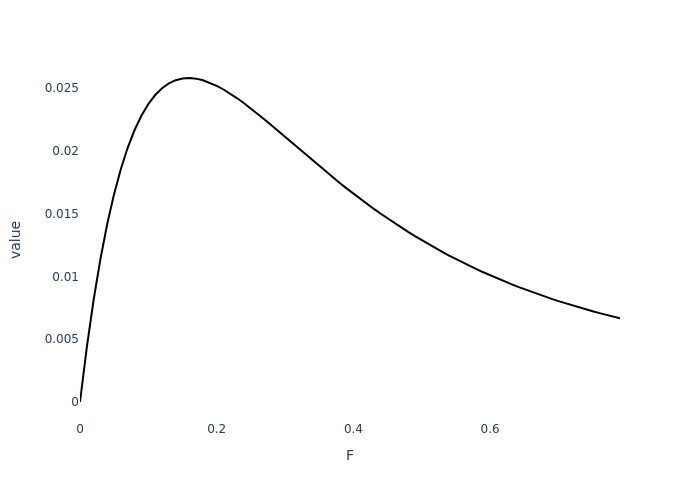
\includegraphics[width=\linewidth]{notebooks/SimpleOptimization/value_v_F.png}
  \caption{Value versus Fishing Mortality}
  \label{fig:value_v_F}
\end{figure}

And boom! This is why optimization is important. Start at $F=0$ and we get an obvious result - if you don't fish you don't get any fish (surprise!). Then as we begin to apply some fishing pressure $F>0$ we can see that the value starts rising rapidly - also expected. However something really interesting happens once we cross $F\approx 0.2$ the value starts to go down! Turns out there is such a thing as too much of a good thing. What's going on here is that after a certain point ramping up the fishing pressure starts to kill so many \textit{young} fish that fish aren't able to grow up into the big chonkers that bring much of the value of the fishery. As a result, the fishery actually becomes poorer as we put more effort into it! More effort screws up the demographics which in turn screws up the fishery. Pretty fascinating if you ask me.  
\newline

Alright, clearly this was a contrived example and part of what made it so easy was our "management" was parametrized by a single variable $F$. This meant that we could just plot out all of the options and choose the best one. In theory, this brute force approach always work. But theory and practice rarely agree on anything and tend to get in fisticuffs over things that were supposed to be the easy part. Practice, you see, suffers from the curse of dimensionality. 
\newline

To illustrate suppose you start with a single parameter case like ours, but one where the parameter is categorical (i.e. it takes on a specific set of values). Maybe that parameter can take on 10 values. This in turn means you need only search $10$ different cases to find your optimal case for sure. 
\newline

Alright, now suppose that you add another 10 value parameter. What comes next can be a little hard to grasp in the abstract, so let's suppose that our first parameter corresponds to the kind of gear used and the second to how many months folks can go out fishing. That means that for each selection of gear we have to independently try each selection of months. This means that rather than having ten cases we have ten times ten cases. Add another parameter (say catch limits per boat) and you now have ten times ten times ten or one thousand cases to check. You can probably see where this is going... in general with $N$ such parameters there are $10^N$ cases to explore!
\newline

This gets computationally inefficient really, really fast. So when folks optimize really large problems (with loads of parameters) they obviously have to turn to things besides brute force search.
\newline

Generally speaking there are two categories - analytic and meta-heuristic. While going into either would take up far too much room here the basic idea behind each is to use knowledge about the solutions you've already looked at to be clever about the next case you choose so you can quickly find better values without having to search the \textit{whole} space. However, nothing comes for free, and so this strategy has a drawback. A pretty darn significant drawback. Except for in a limited number of special cases, these faster strategies don't actually \textit{guarantee} optimality. Instead it's up to you to use them skillfully in order to make the likelihood of finding optimality more and more \textit{probable}. As such it's incredibly important to know what you're using quite intimately to avoid having the wool pulled over your eyes!
\newpage

\noindent \rule{\textwidth}{0.5pt} 
\begin{figure}[h!] 
  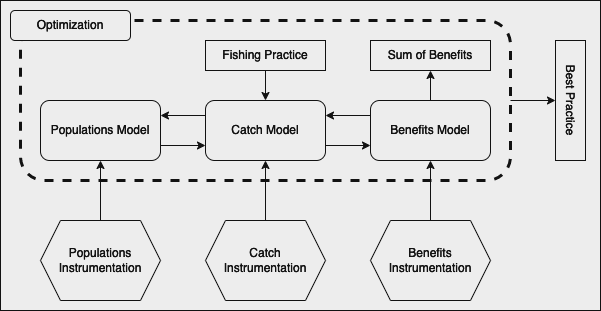
\includegraphics[width=\linewidth]{drawings/high_level.png}
  \caption{30,000ft View}
  \label{fig:high_level}
\end{figure}
\newline
\rule{\textwidth}{0.5pt} 
\vspace{5pt}

At this point we've covered a lot of ground. We've got models that drive our optimization, instrumentation creating the ground truth data used to fit those models, and the optimization itself. Put these together and you can start working toward finding the right set of fishing parameters to maximize the particular balance of benefits presently under consideration. 
\newline

However through all of that something should have become frighteningly clear - all of this is \textit{entirely} dependent on the models used. And so an obvious question comes walking, nay barging - existential sword in hand - through the door - what can go wrong with the modeling itself? We turn to that next. 
\newpage

\chapter{Risky Business}
To understand the things that can go wrong when using predictive models we need a model to poke and prod at. One particularly classic model that's really useful in illustrating some fundamental fisheries concepts is Schaefer's surplus production model. So let's go ahead and use that one to get the most bang for our buck.
\newline

All models are a simplification of reality, it's what makes them both very useful (imagine trying to play god while following every atom in this universe) and rather dangerous (sometimes the details matter in ways you don't expect). Simplification means assumptions that don't necessarily line up perfectly with reality. So let's start with what Schaefer's model assumes. 
\newline

First the model assumes a kind of \textbf{reproductive stability} wherein the number of individuals joining the population each year is precisely the same fraction of the fecund population each and every year. If $P_F$ is the population capable of producing baby fish (the fecund population) and the offspring $P_O$ then this assumption looks like the following in math-speak:

$$P_O = \gamma P_F$$

Now keeping track of two separate populations is a lot of work so the next simplifying assumption the model makes is one of \textbf{demographic stability} wherein the proportion of the population that is fecund remains constant as time rolls on and the population grows and shrinks in response to whatever's going on in the environment. Translating this as well, then if $P$ is the overall population we have:

$$P_F = \alpha P$$

Stability is a wonderful thing so let's go for a triad - \textbf{biomass stability}. This assumption entails making the leap that the average weight per fish is also a constant (given we're assuming demographic stability this isn't actually that much of a leap if you think about it - barring starved fish the average size remaining constant per age group is a pretty commonly held assumption in fisheries science). If the average size per fish is constant than biomass, $B$, and population are more or less indicating the same thing:

$$P = \beta B$$

Combining our three stability assumptions together we get:

$$P_O = \gamma \alpha \beta B \rightarrow B_O = \gamma \alpha B $$

which leads us right into:

$$B_{t+1} = B_{t} + rB_t$$

where $r=\gamma \alpha$ is the growth ratio. 
\newline

\begin{figure}[h!] 
  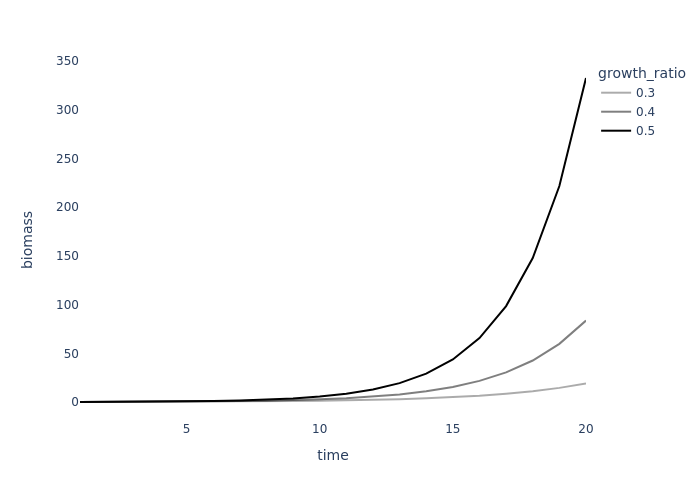
\includegraphics[width=\linewidth]{notebooks/SurplusModels/exponential_growth.png}
  \caption{Unconstrained Growth}
  \label{fig:unconstrained_growth}
\end{figure}

Enough math, let's get a picture! Fig. \ref{fig:unconstrained_growth} shows us what the model would give us for year over year growth and something is clearly wrong - the biomass is rocketing for the stars! That's because this growth is entirely unconstrained it's as if the fish have limitless access to food, space, and have absolutely no predation pressure. No one is dying, no one is hungry - these fish have found utopia!
\newline



Unfortunately the secrets for utopia don't exist in fishy hands and many things prevent this kind of exponential growth. One such concept is the idea of a carrying capacity $B_{\infty}$. This is the point at which the ecosystem has had its full of this particular kind of fish and can take no more. Schaefer's model assumes that this ceiling exerts a kind of linearly increasing pressure on the population that grows so oppressive once the population reaches $B_\infty$ that no more growth is possible at that point. This pressure is defined by a multiplier on our growth ratio $r$ that looks like:

$$(1-B/B_\infty)r$$

To see how this gives our "carrying capacity pressure" consider what happens when $B=0$, at this point we have $(1-0/B_\infty)r=r$ so the growth ratio is able to steam full ahead. As the population grows and we reach $B=B_\infty / 2$ we end up with $(1-1/2)r =0.5r$ - the growth rate coefficient has been reduced to half its true power. Finally when the population does in fact reach the carrying capacity $B=B_\infty$ then we get $(1-1)r=0$ and growth has become impossible. All in all a nice, linear modification in the growth coefficient. We now have:

$$B_{t+1} = B_{t} + (1 - B_t/B_\infty)rB_t$$

\begin{figure}[h!] 
  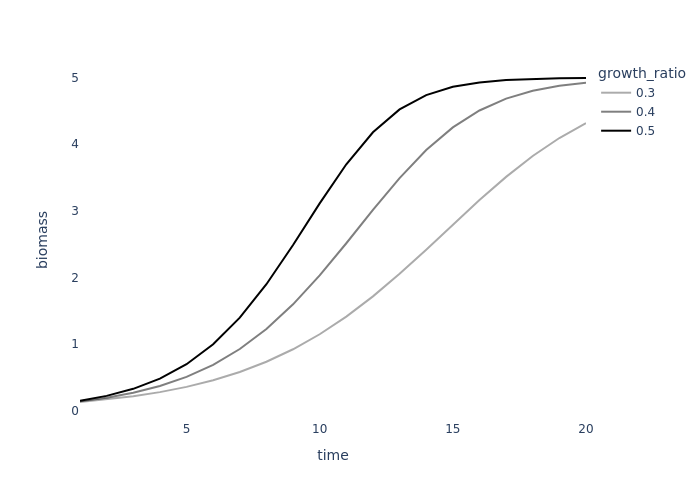
\includegraphics[width=\linewidth]{notebooks/SurplusModels/capped_growth.png}
  \caption{Constrained Growth}
  \label{fig:constrained_growth}
\end{figure}

Fig. \ref{fig:constrained_growth} gives us what happens when we enforce a $B_\infty = 5$ on our prior unconstrained growth curves. Now we can see them leveling out nicely at $B_\infty$ - just as we wanted!
\newline

At this point our fish are gliding up to their carrying capacity, and then, with a fully fledged stable population are contemplating their own mortality as year after year new fish join the population and old ones move onto the fishy beyond. However this peaceful stability is about to end in the sound of diesel engines and the surprise of finding delicious food containing and devastating, hookish surprise. The fishers are on their way!
\newline

Instead of assuming a nice steady fishing mortality like we did last time we're going to assume that these fishers are out to take as much fish as they possible can and are limited only by a fishing cap imposed by us their trust fisheries scientists. So the question now is - what limit should we place? To find out let's model forward with a couple different catch limits. Assuming $r=0.5$ and $B_\infty=5$ we can see what happens in Fig. \ref{fig:adding_the_fishers}.
\newline

\begin{figure}[h!] 
  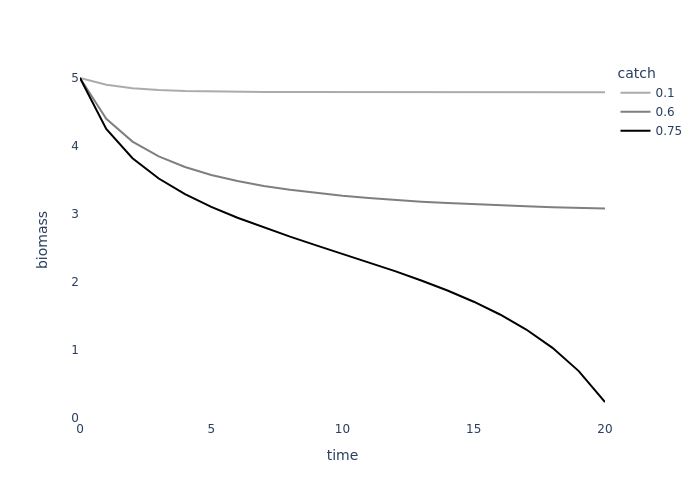
\includegraphics[width=\linewidth]{notebooks/SurplusModels/adding_the_humans.png}
  \caption{Adding the Fishers}
  \label{fig:adding_the_fishers}
\end{figure}

There's a lot to learn from these three curves. We can clearly see that we want to avoid $C=0.75$ the fish stock is clearly on the way to oblivion and our commitment to the long term would vanish like a puff of smoke. However the other two look pretty stable. That being said, $C=0.1$ seems like it's unnecessarily conservative. We catch only a sixth of the fish as in the case of $C=0.6$ yet it's no more stable as both glide into a new happy state of stasis. So why is it that up to a limit we can just fish more and more until suddenly the stock just goes into free fall? How might we tow that line as closely as possible?
\newline

If we turn back to our model we have the following:

$$B_{t+1} = B_t + (1 - B_t/B_\infty)rB_t - C$$

From this we can see that the catch $C$ is competing with the growth $(1 - B/B_\infty)rB$. Let's plot the growth as a function of biomass to see if we can get any hints as to what might be going on (Fig. \ref{fig:growth_v_biomass}).
\newline

\begin{figure}[h!] 
  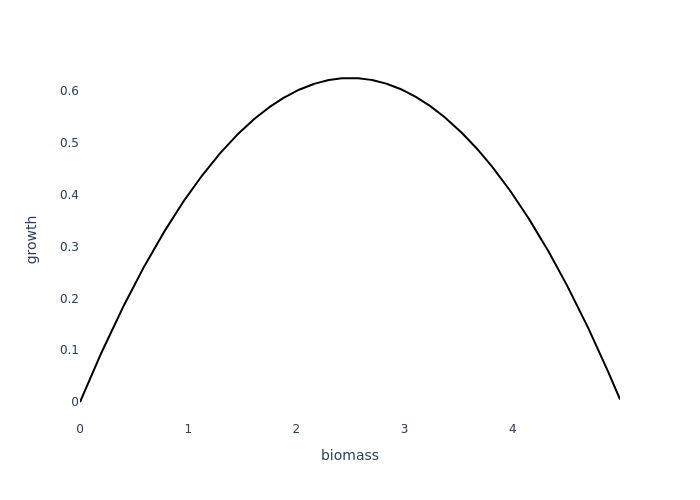
\includegraphics[width=\linewidth]{notebooks/SurplusModels/surplus_yield.png}
  \caption{Growth v Biomass}
  \label{fig:growth_v_biomass}
\end{figure}

Fascinating! The growth has a very clear maximum at precisely $B=B_\infty / 2$. Now we can understand what was changing between our different catch limits. When $C=0.1$ we never put enough pressure to drive the population down to $B=B_\infty / 2$ and so we stayed stuck with our small catch. However when we cranked things all the way up to $C=0.75$ we not only drove our population to $B=B_\infty / 2$ but we missed our exit and went flying past straight toward extinction! No level of biomass could support such a catch with equivalent growth. However at the sweet spot we have a growth of:

$$(1-(B_\infty/2) / B_\infty)r(B_\infty /2) = rB_\infty / 4$$

which happens to be $0.5 \bullet 5 / 4 = 0.625$ in our case. So $C=0.6$ was very nearly the sweet spot!
\newline

In general though, the conclusion we've come to is that under our Schaefer surplus production model the "best" catch is given by $rB_\infty / 4$. In general this "best" catch is called the maximum sustainable yield or MSY. 

$$C_{MSY} = rB_\infty /4$$

Clearly then, for a fishery we didn't just make up (and therefore have all the answers to) we have two parameters we need to fit - $r$ and $B_\infty$. Time to finally find out what can go wrong.

\section{Model Risk}

I'm going to take a leaf out of a wonderful textbook - \textit{Fisheries Biology, Assessment, and Management} by King - and use the example they give to present the Schaefer's surplus production model to instead present just how risky these things can get. 
\newline

Alright so what kind of data do we have from the book? What's our ground truth look like? Fig. \ref{fig:catch_v_effort} shows us what we've got to work with. 
\newline

\begin{figure}[h!] 
  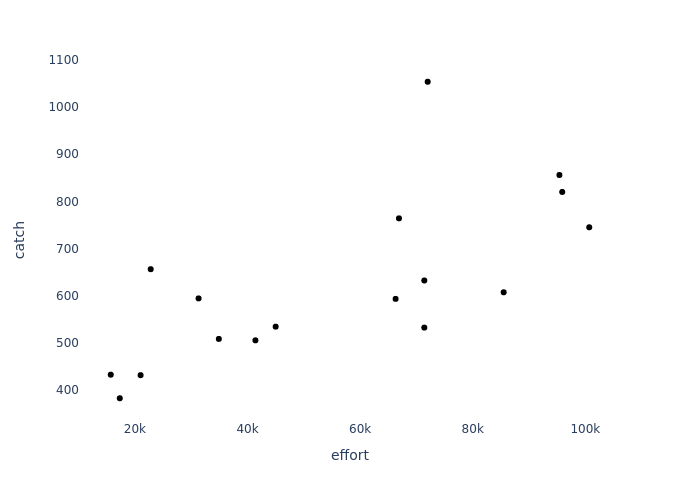
\includegraphics[width=\linewidth]{notebooks/SurplusModels/measurements.png}
  \caption{Catch v Effort}
  \label{fig:catch_v_effort}
\end{figure}

Hmmm... this doesn't seem right at all - we need biomass over time and instead we've got catch versus effort? Well this is a pretty common problem in fisheries science - you want one kind of data but only realize you need it now because you've started doing the fisheries science properly and surprise surprise no one thought to collect that data (or perhaps that data is just impossible to come by - I don't know about you, but measuring every fish in the sea seems like a bit of a monumental task...). 
\newline

Ok, so we've got to work with what we've got. Perhaps there's some assumption we can make to connect these data to what we actually need? Time for a couple more assumptions.
\newline

First we need to introduce the notion of catch per unit effort or CPUE. Effort is usually quantified in something specific to the fishery like number of lobster pots used, time spent out fishing, miles of line used, and so on. Weird but practical. So if effort was, say, miles of line used, the CPUE tells how much catch we can expect from a mile of line. Letting $f$ be the effort we have in math-speak:

$$C = f\bullet CPUE$$

With this concept in mind we can now enter the assumption that's going to allow us to use catch and effort data to fit our surplus model. And that's that the amount of effort required to catch something is directly proportional to the amount of fish in the ocean:

$$CPUE = qB$$

This makes intuitive sense - it becomes easier to catch something the more fish there are to catch. 
\newline

Let's now see how this helps us. Replacing $C$ in our original model with $C=fqB$ we get:

$$B_{t+1} = B_t + (1 - B/B_\infty)rB_T - qf_tB_t$$

Alrighty! We now have four parameters - $r$, $B_\infty$, $B_0$, and $q$ - but can now use our measured fishing effort $f$ to compute the biomass year over year (assuming we know when these catches happened, which lo and behold we do!) and then can use the predicted biomass $B_t$ to predict the catch $C_t = qfB_t$. In other words, given our input variable $f_t$ we can predict our output variable $C_t$ - we can now fit our model! Pretty darn clever. 
\newline

Using a standard optimization library, \textit{scipy.optimize}, from the computing language Python I ended up with $r=0.6766$, $B_\infty = 4001$, $B_0 =2884$, and $q=4.29\bullet 10^{-6}$. From this we can derive our $C_{MSY}\approx 676$.
\newline

Alright, you ask, what's the problem? All of this seems to have gone rather smoothly. Sure, until you look at the data... let's plot the predicted catches vs the actual catches (Fig. \ref{fig:predictions_surplus})
\newline

\begin{figure}[h!] 
  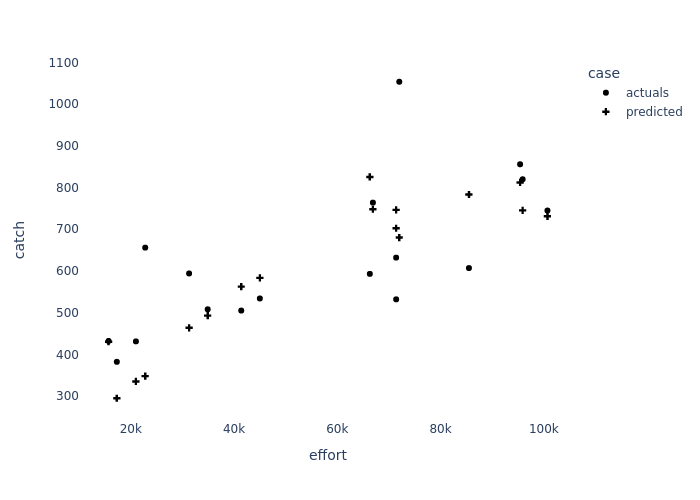
\includegraphics[width=\linewidth]{notebooks/SurplusModels/model_scatter.png}
  \caption{Catch v Effort}
  \label{fig:predictions_surplus}
\end{figure}

My oh my those points are all over the place! Let's compute the distance between the predictions and the actuals (also known as absolutely error) and look at the distribution of the errors (Fig. \ref{fig:predictions_surplus_dist})
\newline

\begin{figure}[h!] 
  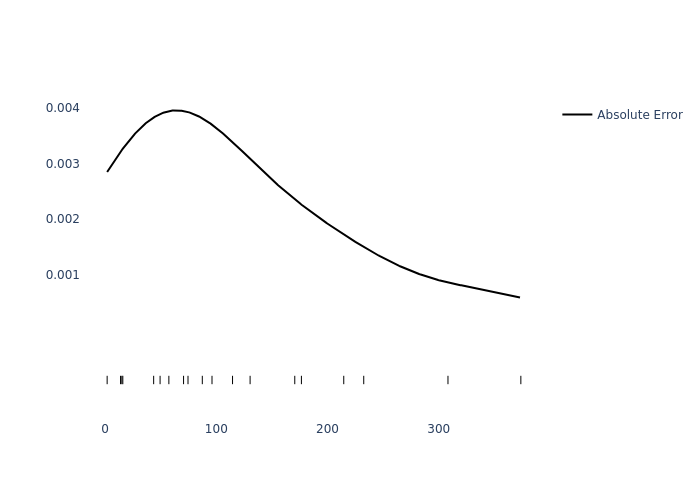
\includegraphics[width=\linewidth]{notebooks/SurplusModels/model_dist.png}
  \caption{Error Distribution}
  \label{fig:predictions_surplus_dist}
\end{figure}

This distribution peaks around 80 or so which is still $>10\%$ of most of our recorded catches! And here, smack dab in front of us is the first kind of risk inherent in modeling - the risk inherent in the fact that our predictions aren't perfect. Every model is like this, because it is a simplification of reality they \textit{never} predict things perfectly accurately. However this inaccuracy has real consequences. 
\newline

For example in our case if we assume we must allow for 10\% error in our predictions then we should allow for an equivalent kind of error in the prediction of $C_{MSY}$, and because overestimating $C_{MSY}$ means a decimated fishery we need to provide estimates that are on the conservative side. But that means telling fishers whose livelihood depend on the catch that for every ten fish they used to catch under our initial estimate that they need to through back 1 and forsake 10\% of their income because our model is not quite hitting the mark. I certainly don't envy the person having to give that news! 
\newline

Obviously then one important quality of a model is how tight those error bars are - the smaller we can shrink the range the less we have to take away from the livelihoods of good folks. However, unfortunately the risk doesn't end there. 

\section{Instrumentation Risk}

So far we've been assuming our ground truth is exactly - the absolute truth. However for anyone who's messed around with scales, taken measurements in a lab, or just generally tried to measure anything you'll know better than to assume this. Even the old adage - measure twice, cut once - comes from a common knowledge that measurements are error prone. 
\newline

This should send a shiver down your spine. Our $r$ and $B_\infty$ are quite dependent on the data we fit to - if that data isn't quite right, neither will be our parameter estimates. And if our parameter estimates are wrong then our $C_{MSY}$ will likely be wrong too... So obviously we need to quantify the risk here too. 
\newline

We can do this by introducing noise into the ground truth data given to us and seeing how it changes our estimates of $C_{MSY}$. Specifically we will randomly shift each ground truth point from the book up or down by 10\%, fit our model, calculate $C_{MSY}$, and repeat until we can get a distribution of possible $C_{MSY}$ values if we assume some error. Fig \ref{fig:instrumentation_error} shows us what we get.
\newline

\begin{figure}[h!] 
  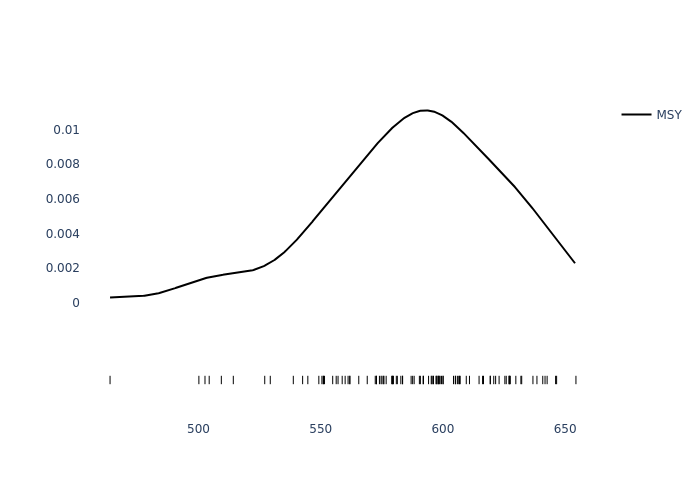
\includegraphics[width=\linewidth]{notebooks/SurplusModels/instrumentation.png}
  \caption{Variation in $C_{MSY}$}
  \label{fig:instrumentation_error}
\end{figure}

Well it's a good thing we checked this! For one thing our original estimate of $C_{MSY}=676$ was actually on the high end! If we wanted to be conservative we clearly need to choose an $C_{MSY}$ closer to 600 which is once again a $\approx 10\%$ reduction in catch and therefore revenue for our fishers. Thinking about the fact that fisheries often get valued in the 10's of millions it makes a lot of sense to improve the instrumentation and therefore shrink these error bars if possible. 10\% of a million is a \textit{lot} of money. 
\newline

\section{Ontological Risk}

So far we've been discussing what can wrong with the modeling process assuming that our model is the right one. However there's a lot of reason to doubt a lot of the assumptions we just made. We assumed demographic stability - if gear selectivity changes year by year this assumption will break down. We assumed that the ease of catch is just a function of biomass - what about technological developments? We also assumed absolutely no randomness in the amount of recruitment that happens each year - what if the fish just have a bad year for some reason? These are all ontological risks - risks associated with making wrong assumptions that lead you to predict things that are just completely and entirely false. 
\newline

As a clear example we're assuming that once a population is at $B=B_\infty / 2$ it will always produce a specific yield of new recruits that we can fish completely. However what if the fish just have a bad year and they aren't able to keep up with our $C_{MSY}$? The result is devastating, they end up falling below that peak growth point and forever more will never be able to keep up with our prescribed fishing pressure and practically start running straight toward oblivion. 
\newline

Another example is the assumption that no matter how small the population gets, it will always try to grow. But we know from research on genetics that there is a smallest population beyond which there simply isn't enough genetic diversity to keep the population alive and healthy. Where is that point? This model has no flipping clue. 
\newline

Ontological risks are the most terrifying because rather than requiring us to be conservative they pose the existential risk that something we're forgetting will drive a population straight into the ground. Therefore ontological risks have to be taken with the utmost seriousness and steps need to be taken to evaluate both the risk and whether it is worth investing in new models and/or instrumentation to just side step the risk entirely and retire some particularly dubious assumptions. 

\section{Reducing Risk}
Alright what's the point of all of this doom and gloom? It's simple, if we were able to remove all risks from our modeling and optimization then we'd just run the fisheries optimization year after year after year and nothing would need to be done. The technical progress in fisheries science is all about reducing these risks. That's why new models, optimizations, and data are introduced - simply to reduce these four kinds of risk:

\begin{enumerate}
\item Model Risk
\item Instrumentation Risk
\item Ontological Risk
\item Optimization Risk
\end{enumerate}

And voila we have a clear way of evaluating and organizing what kinds of technical progress needs to happen within a specific fishery. Identify the risk, categorize it, evaluate its import to the fishery, and then in order of most pressing needs play whack-a-mole. 
\newpage

\chapter{Unparalleled Progress}

I hope at this point it's become apparent just how sprawling these kinds of problems. We've identified at least ten different problems (3 models $\times$ 3 kinds of risk $+$ finding the right kind of optimization) and have to really talk about anything in any real detail - all of our conclusions have been from the relative safety of 30,000ft. In other words - this is a big problem - a big enough problem that no single soul is really going to have a chance at overcoming it. 
\newline

However there's another problem - if you just try to start piling more people in you're quickly going to end up in a too many cooks in the kitchen situation. After 2 or 3 people trying to make the same pot of spaghetti at once is not helping anyone... So what are we to do? Well it turns out that our illustration of just how overwhelming this problem is is part of the solution. To see how let's think about making a sweater.
\newline

Long ago, before the industrial revolution, when you wanted to make a sweater you started with a sheep. Out you'd go to shear a whole bunch of them to get the wool you'd need for sweater. Once the wool is off the sheep you then have to go about first washing it, then spinning it into yarn, and if you were lucky you'd dye it too. At this point you have a bunch of yarn which is pretty great. Now that you have the yarn you're going to grab a pattern and start knitting the sweater itself. After quite a long time you'll then finally have your sweater! 
\newline

As you can imagine this whole process takes many, many months. If you include actually raising the sheep itself the time stretches out to years! And this is because of the simple fact that by making it one, long, holistic process only one person is really working on the sweater at any one time. 
\newline

Now some folks will say that steam power was the greatest outcome from the industrial revolution. However, in my mind, steam's power pales in comparison to the true star development of the industrial revolution - hyper specialization. The reason you can go to a store and get a sweatshirt for \$25 is because that long process we described before was split into components, those components were split into components, and then people over time have driven each of those kinds of work to the utmost limits of efficiency.
\newline

To go back to our cooking example, while it is true that trying to get 8 people to make a single pot of pasta is just going to end up with broken friendships and sore egos, if you divide the pasta making process into going to the grocery store, making the pasta itself from flour and eggs (oh how fancy), prepping the ingredients for the sauce, boiling the pasta itself, and serving the pasta to hungry customers who probably need service as well, then you can easily employ 8 people and be kicking out pasta at a speed that will seem unbelievable to the two trying to do everything by themselves. 
\newline

The key here is that you've divvied the problem into independent components that have very clear interfaces between one another and otherwise don't have to worry about anything outside of their component at all.
\newline

And there's another huge benefit to this kind of specialization. If you're trying to make all the pasta by yourself, do the shopping by yourself, doing the service by yourself, you're probably not going to do any of those things particularly well because you're so busy trying to juggle it all. Master of None as the saying goes. But if all you have to worry about is, say, grocery shopping - then you can pick up loads of grocery shopping tricks. You can start to learn when's the right time to buy certain things, how to provide enough stock to keep things running but not to much that there's unnecessary waste, which stores have the best prices for specific things, and so on. This is a level of detail the generalist can never hope to achieve - certainly not across every single division of their work. So not only do you get more people on the job but those people can innovate on the job \textit{so much more}. 
\newline

And this is why we've spent so much time going over how this fisheries science problem divvies up into different parts and problems. If two or three people can work at a problem at a time then even our 30,000ft view of the divisions means that instead of two or three people on the problem we can have 20 to 30! And the subdividing needn't stop where we've left off - all we've done is provided a formula for subdivision. For example, suppose you're looking at the population modeling component. This can probably be divided itself among recruitment modeling, age to weight modeling, mortality modeling, and so on. And each of these is going to inherit those three risks implicit in the instrumentation, modeling, and ontology. The key is to make sure that whatever the subdivisions they provide the ingredients for specialization - clear interfaces and independence of problems. 
\newline

Which brings me to one last point. Suppose I'm working on trying to improve a recruitment model and I want to evaluate the benefits of what I'm attempting to do. It would be a real bother if I had to pull together a summit of the dozens of folks working on the other components of the problem just to run things through the whole gamut and get a sense of how this effects the "bottom-line" of the fishery. This definitely would put a whole barrier on the independence bit of specialization.
\newline

Instead what I need is to be able to plug my new component into the overall workflow and run it myself. Think of it like being able to pop a new light into your house, flipping the lights on, and seeing whether the new bulb does the trick. If you had to rewire the electrics in the whole house every time, or had to worry about blowing things downstairs with a light bulb upstairs you'd probably rarely (and quite fearfully) try to make any updates. Likewise I need to be able to plug my new model in, flip a switch, and see what effect it makes to the whole. With that in place I can happily go about working on my piece enjoying the independence that powers specialization.
\newline

This then is the goal, to take fisheries modeling, subdivide it into neat, independent components with lovely, abstract, and neat interfaces tied together in a single plug and play workflow that allows dozens of people to work on the same overall problem all at once. 
\newline

Hopefully the outline herein provides a useful place to start. 

\chapter{Questions to Ask Yourself}

\section{Knowing What's There}

\begin{itemize}
\item What are the management parameters?
\item What are the benefits?
\item Who is the society under consideration?
\item How are the benefits balanced?
\item Is this instrumentation or modeling?
\item Which model does this belong to? Population, catch, or benefit?
\item Do the models subdivide into component models? 
\item What are the model inputs, outputs, and parameters?
\item How are they fitting the model?
\item How are they optimizing the management parameters?
\end{itemize}

\section{Knowing What's Not There}
\begin{itemize}
\item What management parameters are missing?
\item What are the risks with this optimization technique?
\item What are the risks with these fitting techniques?
\item What are the instrumentation, model, and ontological risks?
\item What benefits are ignored?
\item How's not represented?
\end{itemize}

\end{document}